\documentclass[tikz]{standalone}

\usetikzlibrary{arrows.meta,positioning}

\begin{document}
	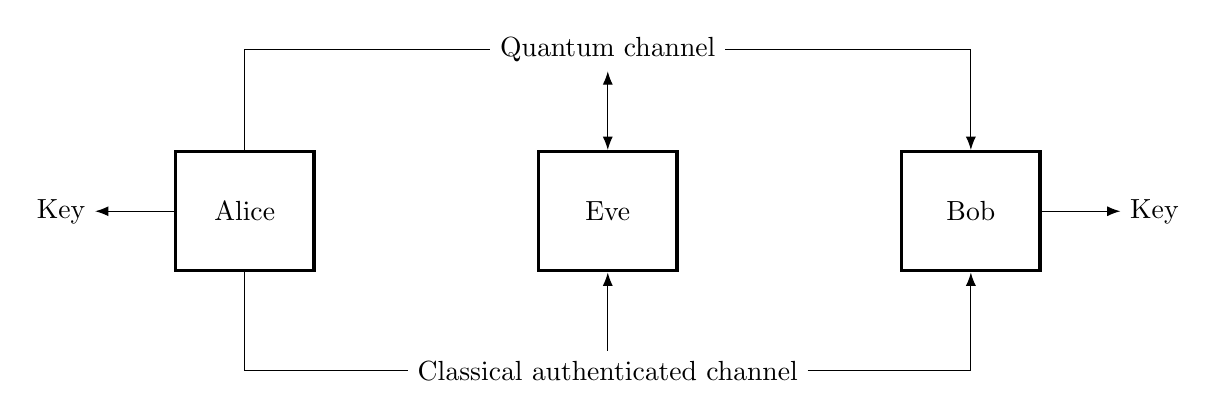
\begin{tikzpicture}[
		block/.style={draw, very thick, fill=white, minimum height=10ex, minimum width=5em},
	]
		\coordinate (in) at (0,0);
		\node (alice) [block, right=of in] {Alice};
		\node (eve) [block, right=8em of alice] {Eve};
		\node (bob) [block, right=8em of eve] {Bob};
		\coordinate[right=of bob] (out);
		
		\node (qch) [above=of eve] {Quantum channel};
		\node (cch) [below=of eve] {Classical authenticated channel};
		
		\draw[-Latex] (alice.north) -- (alice.north|-qch) -- (qch) -- (qch-|bob.north) -- (bob.north);
		\draw[-Latex] (alice.south) -- (alice.south|-cch) -- (cch) -- (cch-|bob.south) -- (bob.south);
		
		\draw[Latex-Latex] (eve) -- (qch);
		\draw[Latex-] (eve) -- (cch);
		
		\draw[-Latex] (bob) -- (out) node[right]{Key};
		\draw[-Latex] (alice) -- (in) node[left]{Key};
	\end{tikzpicture}
\end{document}
